\input ../../SlidePreamble
\input ../../preamble

\begin{document}

{\Huge
  \centerline{\bf TTIC 31230,  Fundamentals of Deep Learning}
  \vfill
  \centerline{David McAllester, Autumn 2021}
  \vfill
  \centerline{\bf 2021 Developments}

\vfill
\vfill

\slide{Wav2vec 2.0, June 2020, Facebook}

Wav2vec pre-trains on audio-only data to get a (discrete) represewntation of speech sounds.

\vfill
Trained on 53k hours of unlabeled audio, and one hour of transcribed audio, Wav2vec outperforms the previous state of the art for 100 hours of transcribed text.


\slide{GLSM, February 2021, Facebook}

This is a speech analogue of a VQ-VAE.

\vfill
Training on audio-only (no text) they convert speech to a sequence of discrete quantized vectors they call pseudo-text units.

\vfill
They then train a generative model of the sequences of pseudo-text units.

\vfill
Semantic and grammatical structure in a ``language model'' is recovered
from speech alone.


\slide{CLIP, January 2021, OpenAI}

CLIP: Contrastive Language-Image Pre-training.

\vfill
Trained on images and associated text (such as image captions or hypertext links to images).

\vfill
The model computes a probability of text given image.

\vfill
It is then used for zero-shot image classification on various datasets.

\vfill
One can classify an image by comparing the probabilities that the model assigns to ``prompts''.  There is a prompt for each class.

\slide{Zero-Shot Image Classification}

\centerline{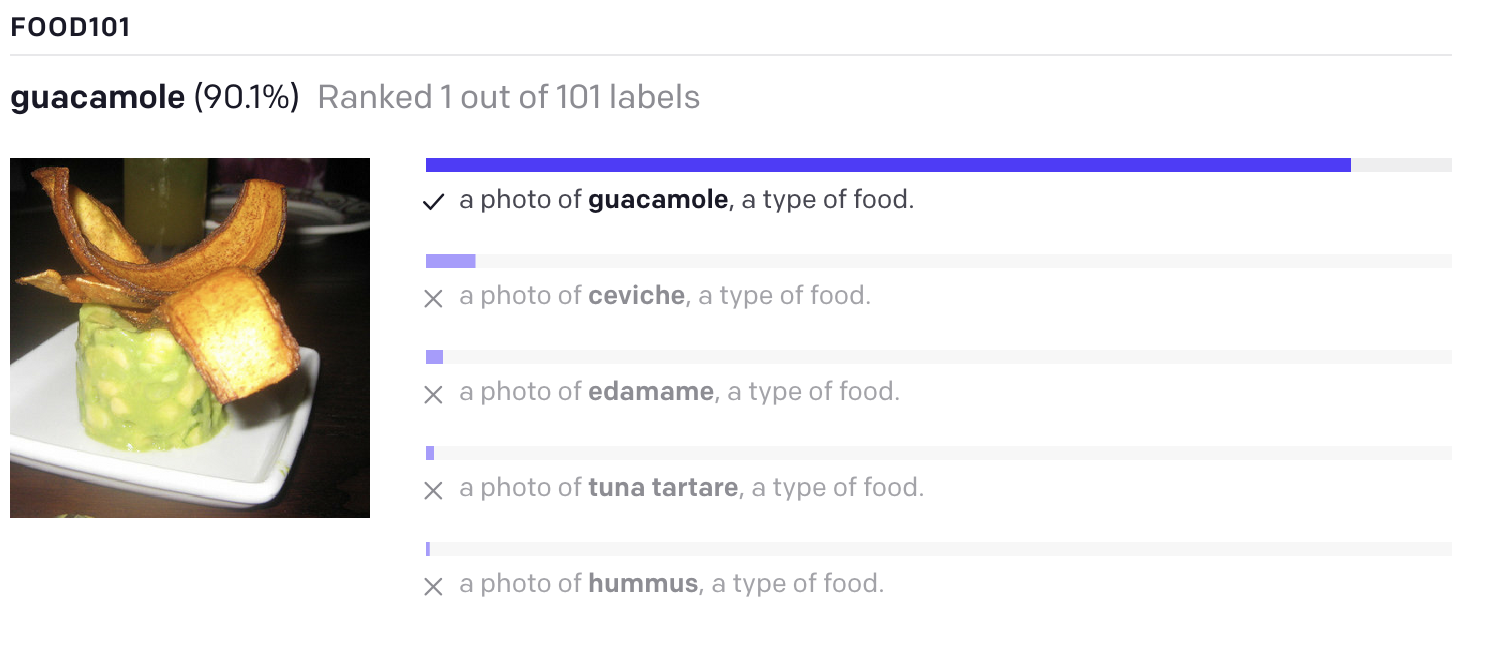
\includegraphics[width = 7in]{\images/CLIP0}}

\slide{Zero-Shot Image Classification}

\centerline{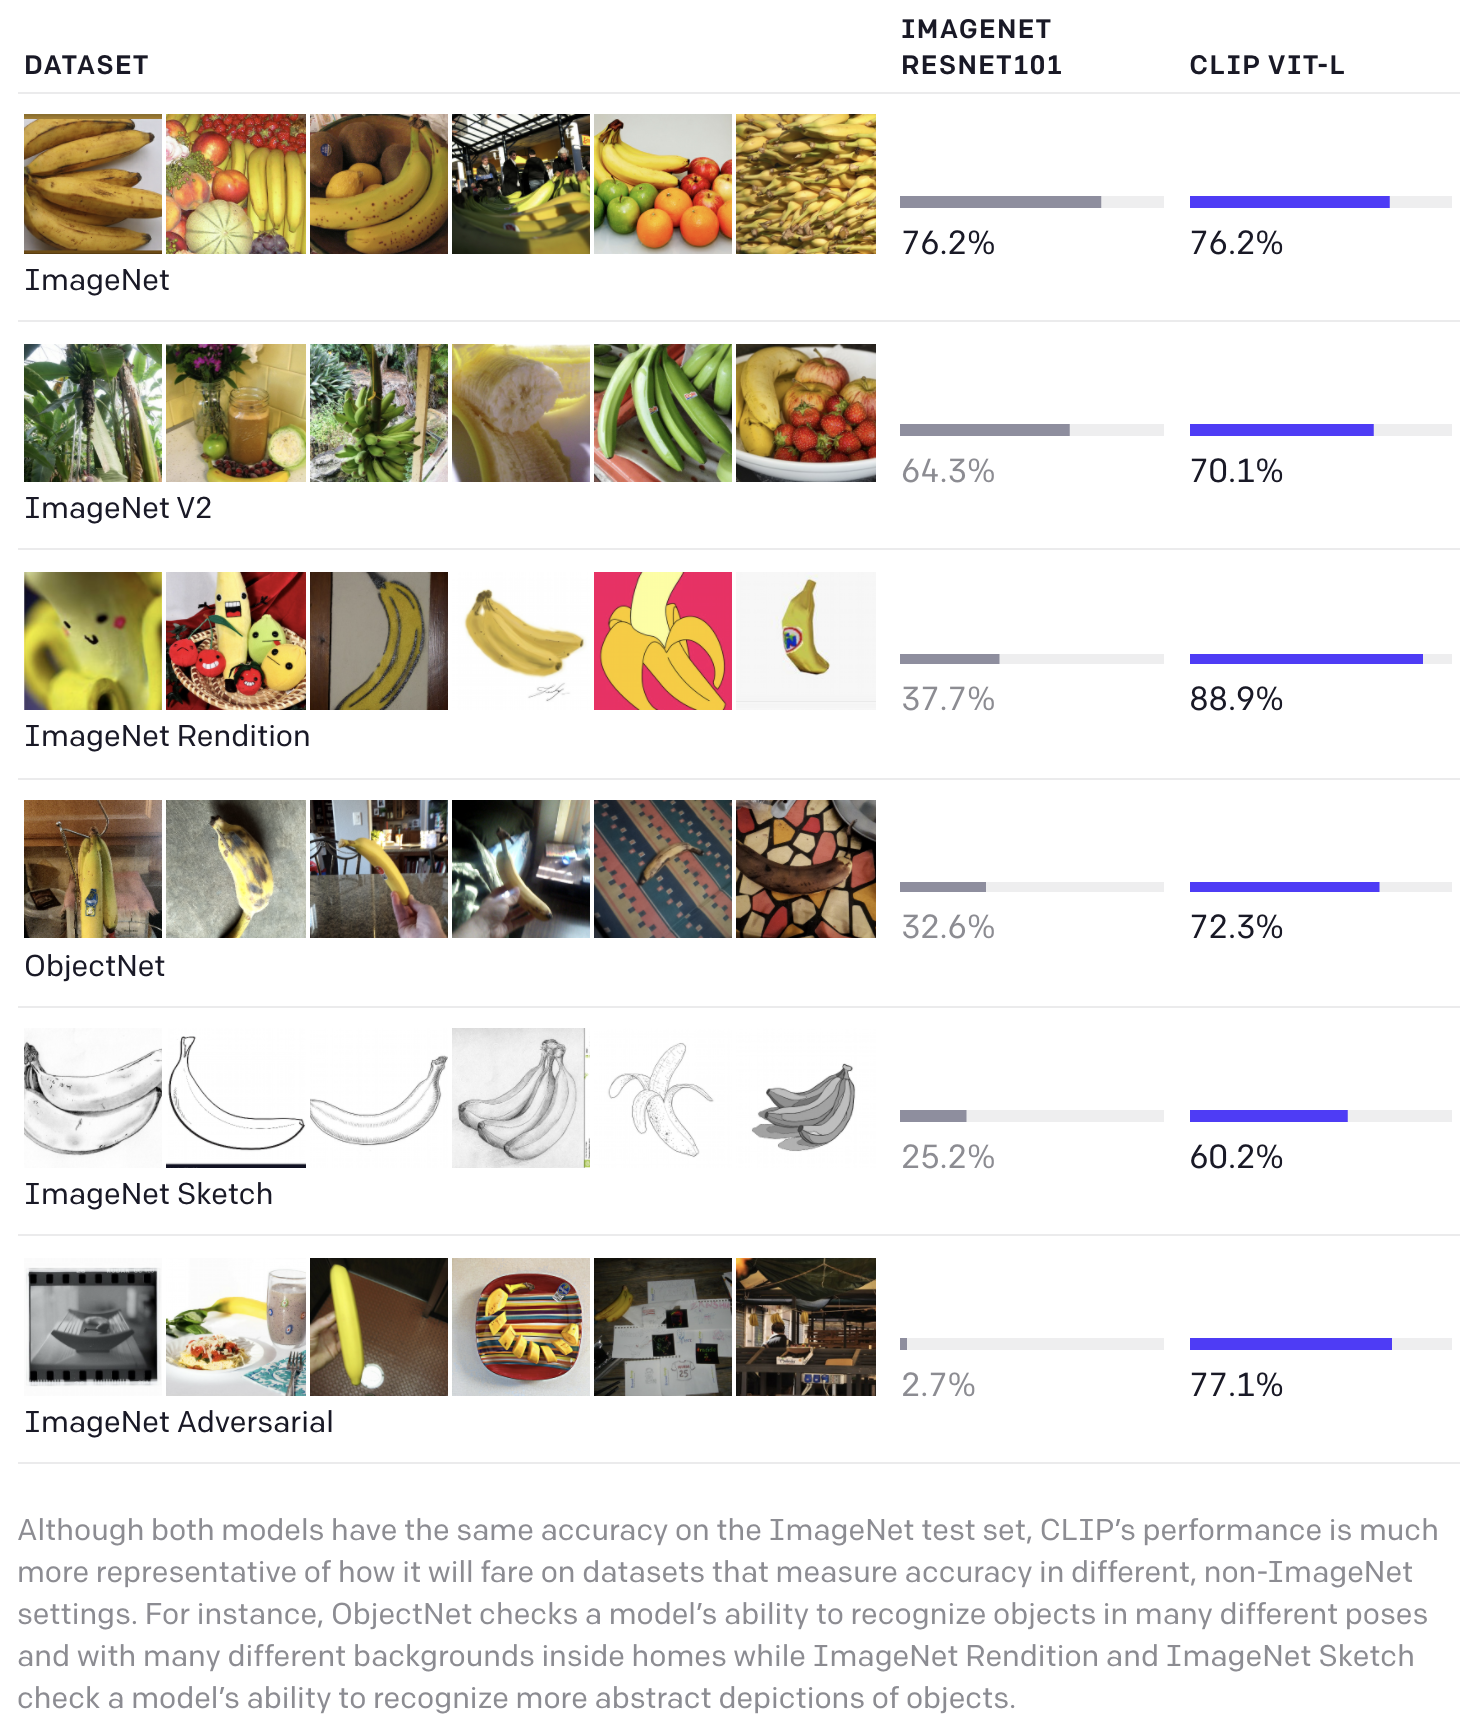
\includegraphics[height= 5in]{\images/CLIP1}}

\slide{DALL$\cdot$E, January 2021, OpenAI}

The name DALL$\cdot$E is simply some kind of homage to the painter Dali and the Disney character WALL$\cdot$E.

\vfill
Like CLIP, DALL$\cdot$E is trained on images paired with text (pressumably the same data as CLIP).  DALL$\cdot$E and CLIP were announced by OpenAI on the same day, although they are different systems.

\vfill
Given text, DALL$\cdot$E generates an image.


\slide{Zero-Shot Image Rendering from Language}

\centerline{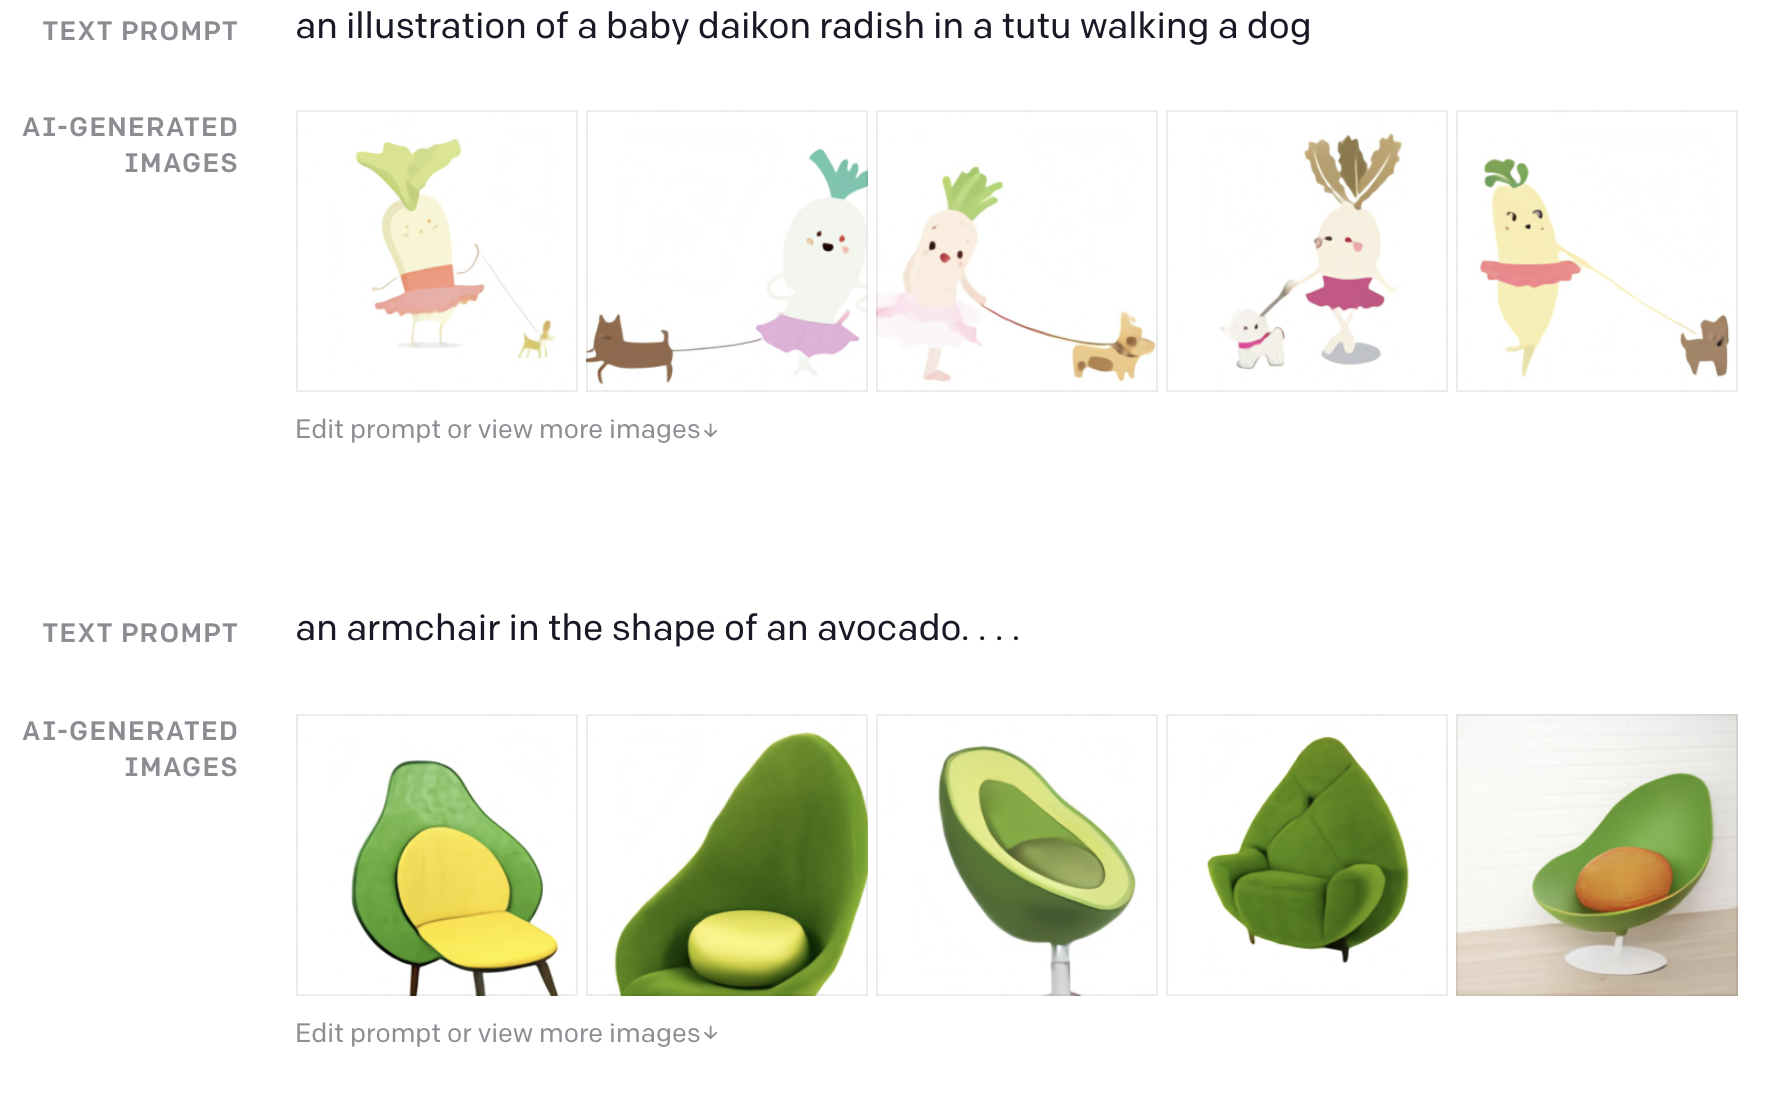
\includegraphics[height= 5in]{\images/DALLE1}}

\slide{Codex, July 2021, OpenAI}

This is a language model trained on code, including comments, from public repositories.

\vfill
Starting from an English prompt Codex continues with code --- a form of automatic programming.

\vfill
There is a published version (58 authors) and a production version that powers GitHub Copilot.

\vfill
Demos indicate a major advance in programmer productivity.

\vfill
This is perhaps a first example of AI being used to bootstrap AI programming.

\slideplain{END}

}
\end{document}
